\part{Análisis estructurado}

\section{Introducción}

\paragraph{Modelo} Descripción simplificada del sistema, que se utiliza en el análisis de requisitos como herramienta sobre la que trabajar con el cliente para construir un sistema adecuado a sus necesidades.\\

Todos los métodos de análisis de requisitos se basan en la construcción de modelos del sistema que se pretende desarrollar, los cuales \textbf{lo reflejan}, mediante la aplicación de \textbf{técnicas de descomposición y de razonamiento \textit{top-down}}. El desarollo de modelos presenta claras \uline{ventajas} como:

\begin{itemize}
    \item \textbf{Ayudar a entender y corregir}:
    \begin{itemize}
        \item Permiten centrarse en determinadas características del sistema.
        \item Permiten realizar cambios y correcciones en los requisitos a bajo coste y sin correr ningún riesgo. Si no se realizasen modelos, estos cambios solo se efectuarían después de construir el producto software.
    \end{itemize}
    \item \textbf{Ayudar a representar y transmitir}:
    \begin{itemize}
        \item Permiten verificar que el ingeniero del software ha entendido correctamente las necesidades del usuario, y que las ha documentado de forma que los diseñadores y programadores puedan construir el software.
    \end{itemize}
    \item \textbf{Ayudar en el proceso de reflexión} (\textit{feedback}):
    \begin{itemize}
        \item Permiten comprobar la correcta realización de cada fase determinando si verifican o no los modelos.
    \end{itemize}
\end{itemize}

\subsection{Problemas del análisis clásico}

No todas las técnicas de análisis logran estos objetivos. Por ejemplo, una descripción del sistema de 500 páginas ocultará características del sistema, tendrá un desarrollo enormemente costoso, y será difícil de modificar, entre otros motivos.\\

Esto se ve claramente reflejado en el análisis de requisitos clásico, usado hasta finales de los 70. Este consistía en redactar especificaciones funcionales, en forma de documentos de texto que eran:

\begin{enumerate}
    \item \textbf{Monolíticos}: Había que leerlos de principio a fin.
    \item \textbf{Redundantes}: Lo cual suele inducir a inconsistencias en caso de querer hacer cambios.
    \item \textbf{Ambiguas}: Por el uso del lenguaje natural.
    \item \textbf{Imposibles de mantener o modificar}: Al ser redundantes, cualquier modificación de una parte podía provocar una inconsistencia, obligando a leer todo el documento debido a que era una ``unidad monolítica''.
\end{enumerate}

Es por ello que la mayor parte del software de la época carece de documentación fiable.

\subsection{Soluciones al análisis clásico}

Como consecuencia, fueron surgiendo nuevos métodos de análisis con los que obtener especificaciones:

\begin{enumerate}
    \item \textbf{Gráficas}: Diagramas acompañados de información textual detallada. Sirven únicamente como material de referencia, y no de cuerpo principal de la especificación.
    \item \textbf{Particionadas}.
    \item \textbf{Mínimamente redundantes}.
    \item \textbf{Transparentes}: Fáciles de leer y comprender.
\end{enumerate}

%Lo siento mucho almuiña pero aquí es probable que pregunte por siglas
\section{Técnicas de especificación y modelado}

El análisis estructurado \textbf{propone la descripción de los sistemas según tres puntos de vista} (como si fuesen tres dimensiones del espacio):

\begin{enumerate}
    \item \textbf{Punto de vista de los datos (dimensión de la información)}: Se centra en la información que utiliza el sistema, representando el modelo de los datos usados, así como las relaciones entre ellos. Algunos ejemplos son:
          \begin{itemize}
              \item \textbf{D}iagramas \textbf{E}ntidad--\textbf{R}elación (\textbf{DER}).
              \item \textbf{D}iagramas \textbf{E}structura de \textbf{D}atos (\textbf{DED}).
          \end{itemize}
    \item \textbf{Punto de vista del proceso (dimensión de la función)}: Se centra en qué hace el sistema, describiendo el conjunto de operaciones que reciben flujos de datos de entrada, y los transforman en flujos de datos de salida. Algunos ejemplos son:
          \begin{itemize}
              \item \textbf{D}iagramas de \textbf{F}lujo de \textbf{D}atos (\textbf{DFD}).
              \item \textbf{Especificaciones de Procesos} (\textbf{PSPECs}): Término genérico que engloba la definición de cómo un sistema transforma unas entradas en salidas mediante pseudocódigo, lenguaje natural, diagramas de flujo\ldots
          \end{itemize}
    \item \textbf{Punto de vista del comportamiento (dimensión del tiempo)}: Se centra en cuándo sucede algo en el sistema, modelando el sistema como una sucesión de estados o modos de funcionamiento, así como se indica cuáles son las condiciones o eventos que hacen que el sistema pase de un modo a otro. Algunos ejemplos son:
          \begin{itemize}
              \item \textbf{D}iagramas de \textbf{F}lujo de \textbf{C}ontrol (\textbf{DFC}).
              \item \textbf{Especificaciones de Control} (\textbf{CSPECs}).
              \item Diagramas de Estados.
              \item Redes de Petri.
          \end{itemize}
\end{enumerate}

\textbf{Nota:} \textit{Todos los modelos describen el mismo sistema, pero desde distintos puntos de vista. Por ende, debe asegurarse la consistencia ellos.}\\

Cada sistema en particular tendrá una \uline{representación de mayor o menor importancia para cada una de estas dimensiones}. Por ejemplo, un sistema de información basado en una gran base de datos, tendrá una importante componente en la dimensión de la información; un sistema de gestión en tiempo real, tendrá mayor peso en la dimensión del tiempo; y un sistema de simulación, hará mayor énfasis en la dimensión de la función.\\

Al final, \textbf{cada modelo se centra en un número limitado de aspectos del sistema}, dejando de lado otros, y será necesario \textbf{combinar todos los que se consideren necesarios para tener una visión detallada} de todas las características del sistema.\\

Por otra parte, la relación entre los diagramas de cada dimensión se establece con las técnicas que representan los planos formados por cada dos dimensiones.\\

En la tabla siguiente se representa una posible clasificación de las \uline{técnicas de modelado} según su/sus dimensiones; las que tengan la misma fila y columna, se centrarán en una dimensión, mientras que las otras harán referencia al plano formado por las dos dimensiones indicadas por su fila y columna.

\begin{table}[ht]
    \centering
    \resizebox{\textwidth}{!}{
        \begin{tabular}{c|l|l|l|} \cline{2-4}
                                                                        & \multicolumn{1}{c|}{\textbf{Información}} & \multicolumn{1}{c}{\textbf{Función}} & \multicolumn{1}{|c|}{\textbf{Tiempo}} \\ \hline

            \multicolumn{1}{|c|}{\multirow{4}{*}{\textbf{Información}}} & D. entidad--relación                      &                                      &                                       \\
            \multicolumn{1}{|c|}{}                                      & D. de estructura de datos                 &                                      &                                       \\
            \multicolumn{1}{|c|}{}                                      & Matriz entidad/entidad                    &                                      &                                       \\
            \multicolumn{1}{|c|}{}                                      & D. de clases                              &                                      &                                       \\ \hline

            \multicolumn{1}{|c|}{\multirow{7}{*}{\textbf{Función}}}     & D. de flujo de datos                      & D. de flujo de datos                 &                                       \\
            \multicolumn{1}{|c|}{}                                      & Matriz función/entidad                    & D. de casos de uso                   &                                       \\
            \multicolumn{1}{|c|}{}                                      & D. de clases                              & D.de estructura de datos             &                                       \\
            \multicolumn{1}{|c|}{}                                      & D. de colaboración                        & Tarjetas CRC                         &                                       \\
            \multicolumn{1}{|c|}{}                                      &                                           & D. de componentes                    &                                       \\
            \multicolumn{1}{|c|}{}                                      &                                           & D. de despliegue                     &                                       \\
            \multicolumn{1}{|c|}{}                                      &                                           & D. de actividad                      &                                       \\ \hline

            \multicolumn{1}{ |c| }{\multirow{4}{*}{\textbf{Tiempo}}}    & D. de historia y vida de la entidad       & Redes de Petri                       & D. de flujo de control                \\
            \multicolumn{1}{|c|}{}                                      & D. de estados                             & D. de estados                        & D. de estados                         \\
            \multicolumn{1}{|c|}{}                                      & D. de secuencia                           & D. de secuencia                      &                                       \\
            \multicolumn{1}{|c|}{}                                      &                                           & D. de actividad                      &                                       \\ \hline
        \end{tabular}
    }
    \caption{Diferentes técnicas de modelado}
\end{table}

Dichas técnicas buscan modelar a alto nivel el sistema en cada una de sus dimensiones.\\

Las siguientes técnicas dan el máximo nivel de detalle posible de aquel aspecto que representan, por lo que se conocen como \uline{técnicas de especificación}.

\begin{table}[ht]
    \centering
    \resizebox{\textwidth}{!}{
        \begin{tabular}{c|l|l|l|} \cline{2-4}
                                                                        & \multicolumn{1}{c|}{\textbf{Información}} & \multicolumn{1}{c}{\textbf{Función}} & \multicolumn{1}{|c|}{\textbf{Tiempo}} \\ \hline

            \multicolumn{1}{|c|}{\multirow{1}{*}{\textbf{Información}}} & Especificación de entidad                      &                                      &                                       \\ \hline

            \multicolumn{1}{|c|}{\multirow{3}{*}{\textbf{Función}}}     &                                           & Diccionario de datos                 &                                       \\
            \multicolumn{1}{|c|}{}                                      &                                           & Especificación de procesos                   &                                       \\
            \multicolumn{1}{|c|}{}                                      &                                           & Especificación de entidades externas            &                                       \\ \hline

            \multicolumn{1}{ |c| }{\multirow{1}{*}{\textbf{Tiempo}}}    &                                           & Definición de función                       & Especificación de eventos                \\ \hline
        \end{tabular}
    }
    \caption{Diferentes técnicas de especificación}
\end{table}


\subsection{Diagramas de flujo de datos (DFD, Función--Información, Función--Función)}

Surgen como respuesta a la necesidad de describir:

\begin{itemize}
    \item \textbf{Qué funciones} son las que realiza el sistema.
    \item \textbf{Qué interacción} se produce entre estas funciones: A dónde va la información de salida de una determinada función.
    \item \textbf{Qué transformaciones de datos} realiza el sistema, especificando \textbf{qué datos de entrada se transforman en qué datos de salida}: Qué se convierte en qué, y por dónde va.
\end{itemize}

Así, el \textbf{DFD} representa el \uline{flujo de información} y las \uline{transformaciones} que se aplican a los datos al moverse desde la entrada a la salida. Dicho de otro modo, se representa el sistema desde un \textbf{punto de vista funcional}; esto es, las \textbf{entidades básicas son funciones o procesos} que transforman unos datos de entrada en salidas, y el sistema resulta ser el flujo de información a través de estas funciones.\\

Los DFD \textbf{NO} representan el \textbf{comportamiento del sistema}, ni el \textbf{control del mismo}; es decir, solo dicen lo que hace el sistema pero \textbf{NO} indican:

\begin{enumerate}
    \item \textbf{Cuándo se hace}.
    \item \textbf{En qué secuencia se hace}.
\end{enumerate}

\subsubsection{Elementos}

\begin{figure}[H]
    \centering
    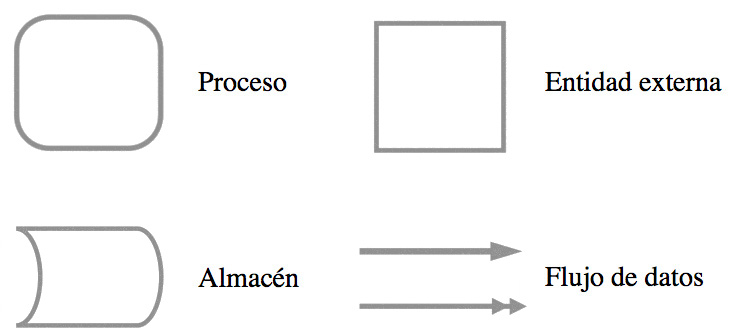
\includegraphics[width=0.5\linewidth]{Resources/Tema5/elementosDFD.jpg}
    \caption{Notación utilizada para representar los elementos de un DFD.}
    \label{fig:elementosDFD}
\end{figure}
\begin{enumerate}
    \item \textbf{Procesos}: Representan elementos software que \uline{transforman información}; por ende, son los componentes del software que realizan cada una de las \uline{funciones del sistema}. Deben verificar las siguientes \uline{reglas}:
    \begin{itemize}
        \item \textbf{De conservación de datos}: El proceso debe ser capaz de generar las salidas a partir de los flujos de entrada más una posible información local.
        \item \textbf{Pérdida de información}: Todas las entradas del proceso tienen que emplearse para calcular alguna de sus salidas.
    \end{itemize}

    \item \textbf{Entidades externas}: Representan elementos del sistema informático o de otros sistemas adyacentes (en todo caso, fuera del los límites del sistema software) que producen información que será transformada por el software, o consumen la resultante. Los flujos de datos que comunican el sistema con las entidades externas representan las interfaces del sistema. \textbf{Sólo pueden aparecer en el diagrama de contexto}, y los flujos entre unidades externas no son objeto de estudio.

    \item \textbf{Almacenes de datos}: Representan información almacenada que puede ser utilizada por el software; concretamente, permiten guardar de forma temporal información que será consumida, o bien por el mismo proceso que la creó, o bien por otro distinto; en la mayoría de los casos, se utilizarán almacenes de datos cuando los \uline{procesos intercambien información pero no estén sincronizados}. Se pueden representar múltiples veces para una mayor legibilidad, y no pueden existir comunicaciones entre almacenes.

    \item \textbf{Flujos de datos}: Representan \uline{datos o colecciones de datos que fluyen a través del sistema}, conectando los procesos con otros procesos, con entidades externas o con almacenes de datos. Posiblemente, en los diagramas de nivel mayor existirán flujos de datos bidireccionales (\uline{par de diálogo}), o incluso varios flujos de datos agrupados en uno solo (\uline{flujos múltiples}), que serán refinados en sucesivos diagramas. Contienen información de las tres dimensiones, aunque normalmente sólo representan las dimensiones de Función e Información. Aún así cabe destacar que, según su \textbf{dimensión temporal}, los flujos pueden ser:
          \begin{enumerate}[a.]
              \item \textbf{Discretos} \textit{(flecha con una cabeza)}: Representan movimiento de datos en un instante determinado de tiempo.
              \item \textbf{Continuos} \textit{(flecha con dos cabezas)}: Implican una transmisión continua de información; \textit{por ejemplo: comprobar si un registro ha cambiado}.
          \end{enumerate}
\end{enumerate}

\textbf{Nota:} \textit{La comunicación entre almacenes y entidades externas solo se representará excepcionalmente cuando el almacén haga de interfaz con la entidad.}

\begin{figure}[h!]
    \centering
    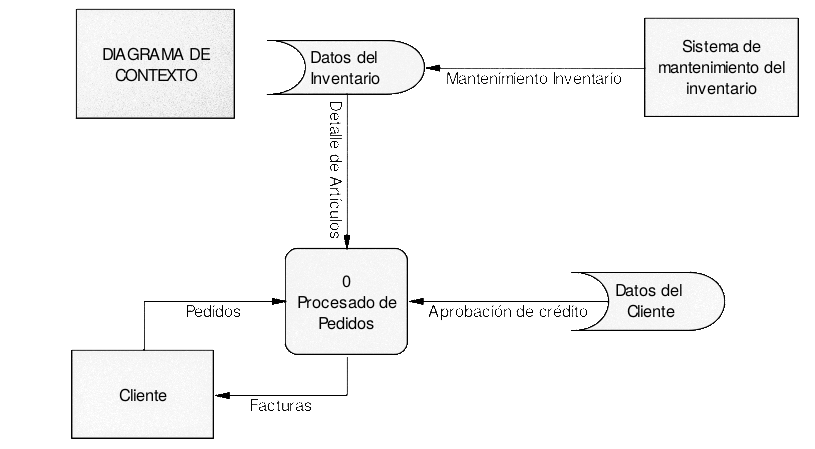
\includegraphics[width=0.8\linewidth]{Resources/Tema5/ejemploDFDInterfazAlmacen.png}
    \caption{Ejemplo de un Diagrama de Flujo de Datos en el que un almacén actúa de interfaz con una entidad.}
    \label{fig:ejemploDFDInterfazAlmacen}
\end{figure}

Cualquiera de los elementos de un DFD tiene que estar etiquetado con un nombre significativo y único:

\begin{itemize}
    \item Los procesos y entidades externas se etiquetan con la función que realizan.
    \item Los flujos de datos se etiquetan con un nombre identificativo de la información, e incluso su estado. \textit{Por ejemplo: número de teléfono, número de teléfono correcto, número de teléfono incorrecto\ldots}
    \item Los almacenes de datos se etiquetan con un nombre significativo de la información contenida, generalmente en plural.
\end{itemize}

\subsubsection{Niveles}

Los \textbf{DFD} permiten la representación del sistema en múltiples niveles de abstracción, de modo que se pueden representar gráficos con un número reducido de procesos (como máximo 7$\pm$2), y con un límite ideal de 7--8 niveles; si fuese necesario emplear más niveles, o bien la complejidad del sistema sería muy alta, o bien el desarrollador está descomponiendo demasiado sus características. Cabe distinguir:

\begin{enumerate}
    \item \textbf{Nivel 0}: \textbf{Diagrama de Contexto}.\\
          Representa el sistema como un único proceso, el \textbf{proceso 0}, que realiza la función principal del sistema, como si de una \uline{caja negra} se tratase. Se representan también las entidades que interactúan con el mismo, dejando claros los \textbf{límites del sistema}, así como sus \textbf{interfaces}.\\
          
          A partir de este diagrama de contexto, se pueden ir construyendo nuevos diagramas que vayan \textbf{definiendo con mayor nivel de detalle el sistema} ya que, en general, un proceso que aparezca en un DFD puede ser descrito más detalladamente con un nuevo DFD; a este procedimiento se le llama \uline{explosión de un proceso}. Así, el proceso aparece descompuesto en una serie de subprocesos o subsistemas. Los flujos de datos que entraban y salían del proceso deben hacerlo también del DFD que lo desarrolla, y este contendrá por lo general nuevos flujos que comunican los procesos que figuren en él, y posiblemente almacenes de datos.\\

          \textbf{Nota:} \textit{Las entidades externas solo aparecen, por lo tanto, en el DFD de contexto.}

          %Imagen nivel 0
          \begin{figure}[h!]
              \centering
              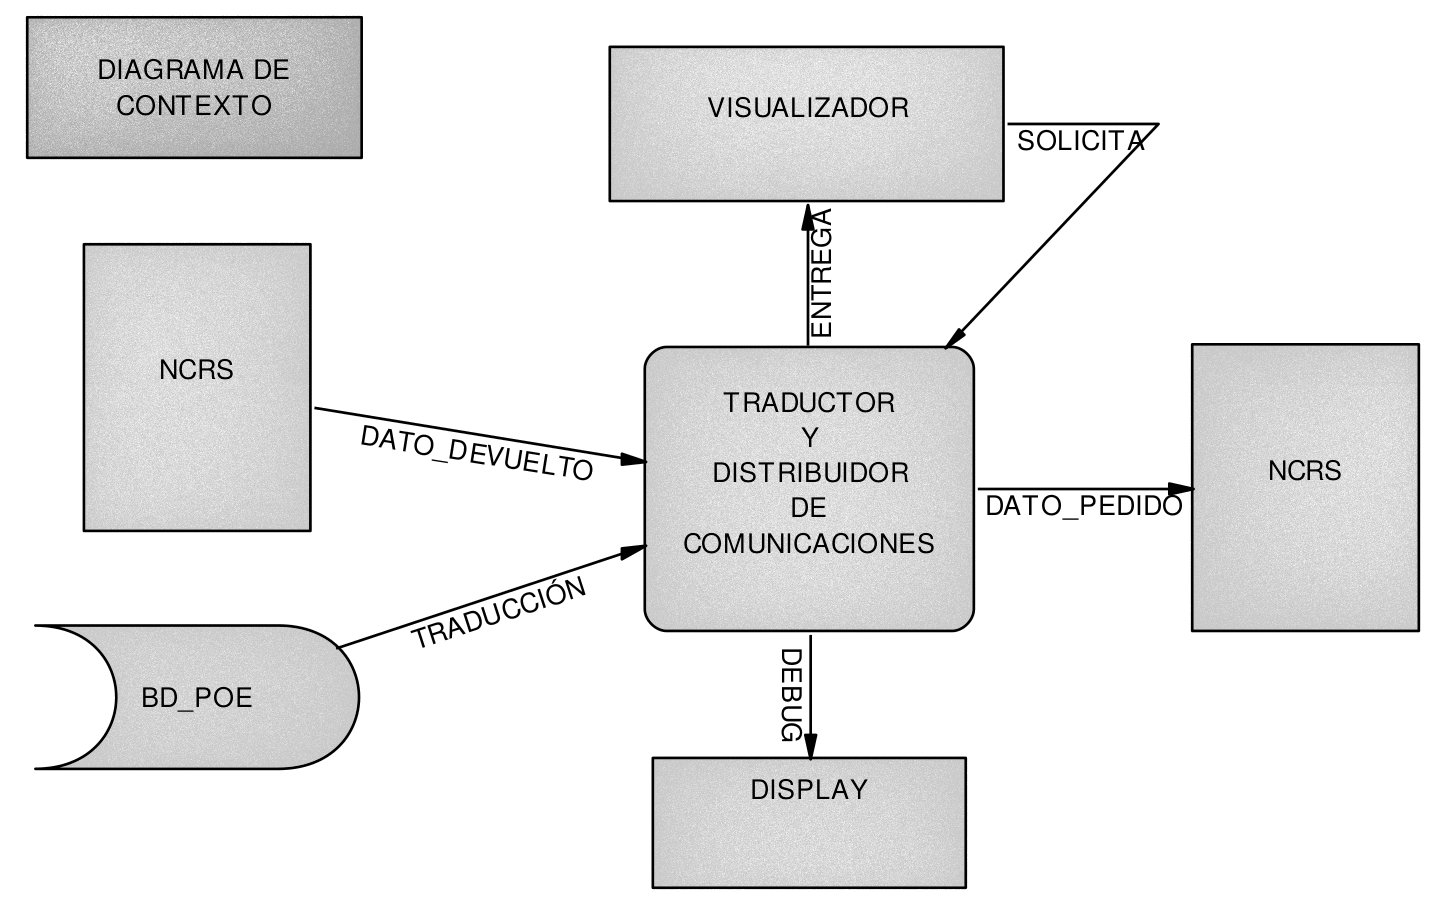
\includegraphics[width=0.7\linewidth]{Resources/Tema5/nivel0.png}
              \caption{DFD de nivel 0 de un Traductor y Distribuidor de Comunicaciones (TDC). Nótese cómo se respetan las posiciones explicadas en el anterior tema para un diagrama del contexto; \textit{por ejemplo: NCRS se muestra tanto como productor como consumidor de información}.}
              \label{fig:dfdn0}
          \end{figure}
    \item \textbf{Nivel 1}: \textbf{Diagrama 0} o \textbf{de Sistema}.\\
          Denominado así por \uline{descomponer el proceso 0} en sus funciones principales; es interesante que estas sean \uline{independientes} y que procesen \uline{los mismos flujos} que el de nivel 0.
          %Imagen nivel 1
          \begin{figure}[h!]
              \centering
              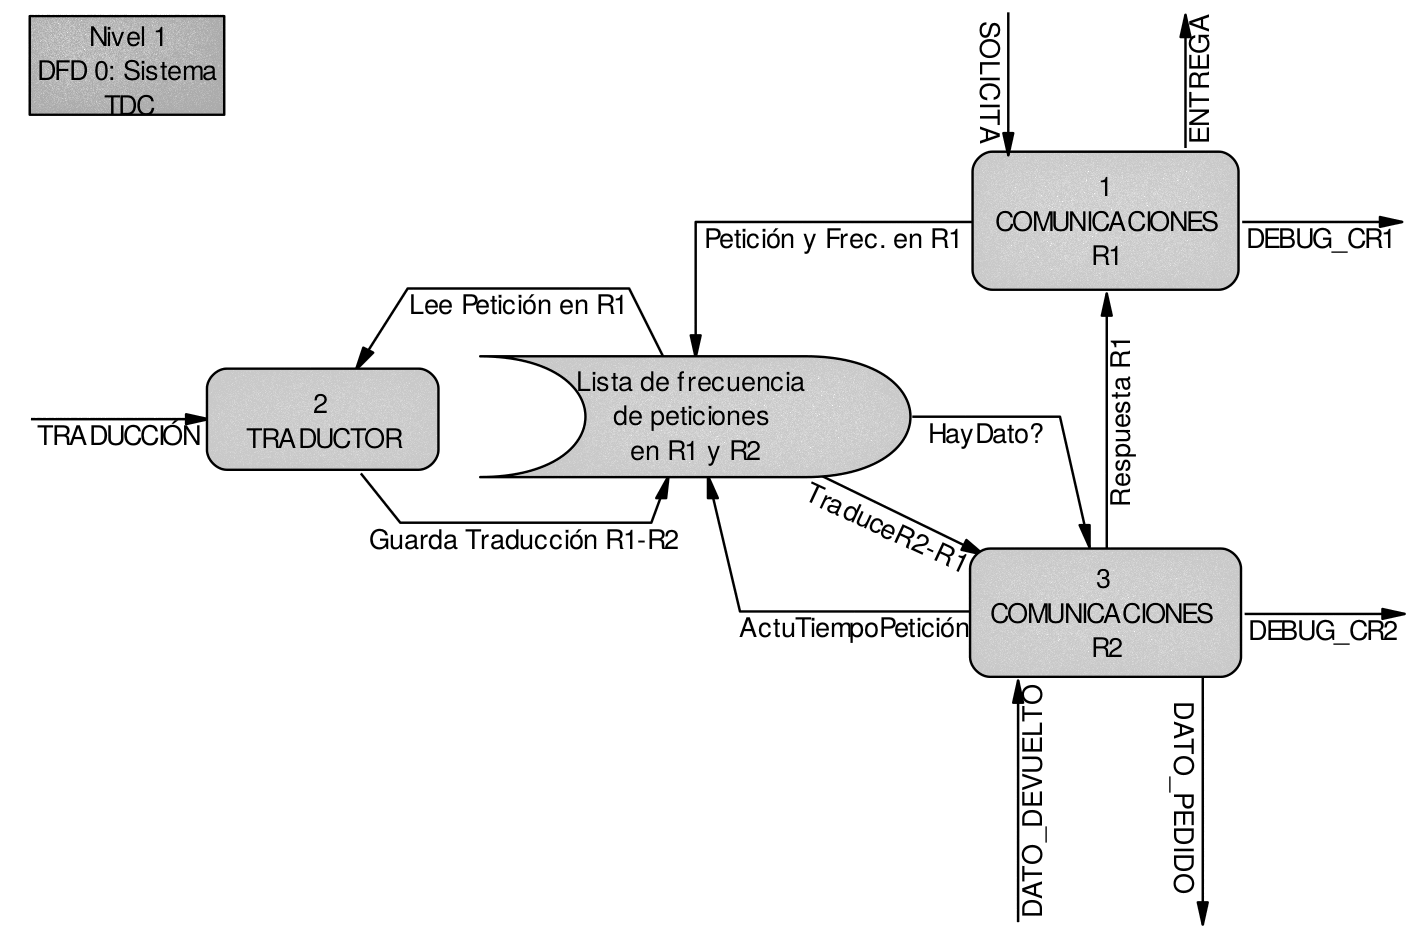
\includegraphics[width=0.7\linewidth]{Resources/Tema5/nivel1_DFD.png}
              \caption{DFD de nivel 1 del TDC. Nótense los flujos de control \textit{DEBUG\_CR1} y \textit{DEBUG\_CR2}, que denotan que procedían de un flujo compuesto situado en un diagrama antecesor. Por otra parte, es habitual que el significado de las posiciones empiece a perderse tras el DFD de nivel 0, priorizando ahora el situar los elementos en donde sea más conveniente.}
              \label{fig:dfdn1}
          \end{figure}
    \item \textbf{Niveles 2...N--1}\\
          Se continúa descomponiendo los procesos en subprocesos, recogiendo las interfaces (flujos) de nivel superior y asignándoselas a subprocesos.
          %Imagen nivel 2
          \begin{figure}[h!]
              \centering
              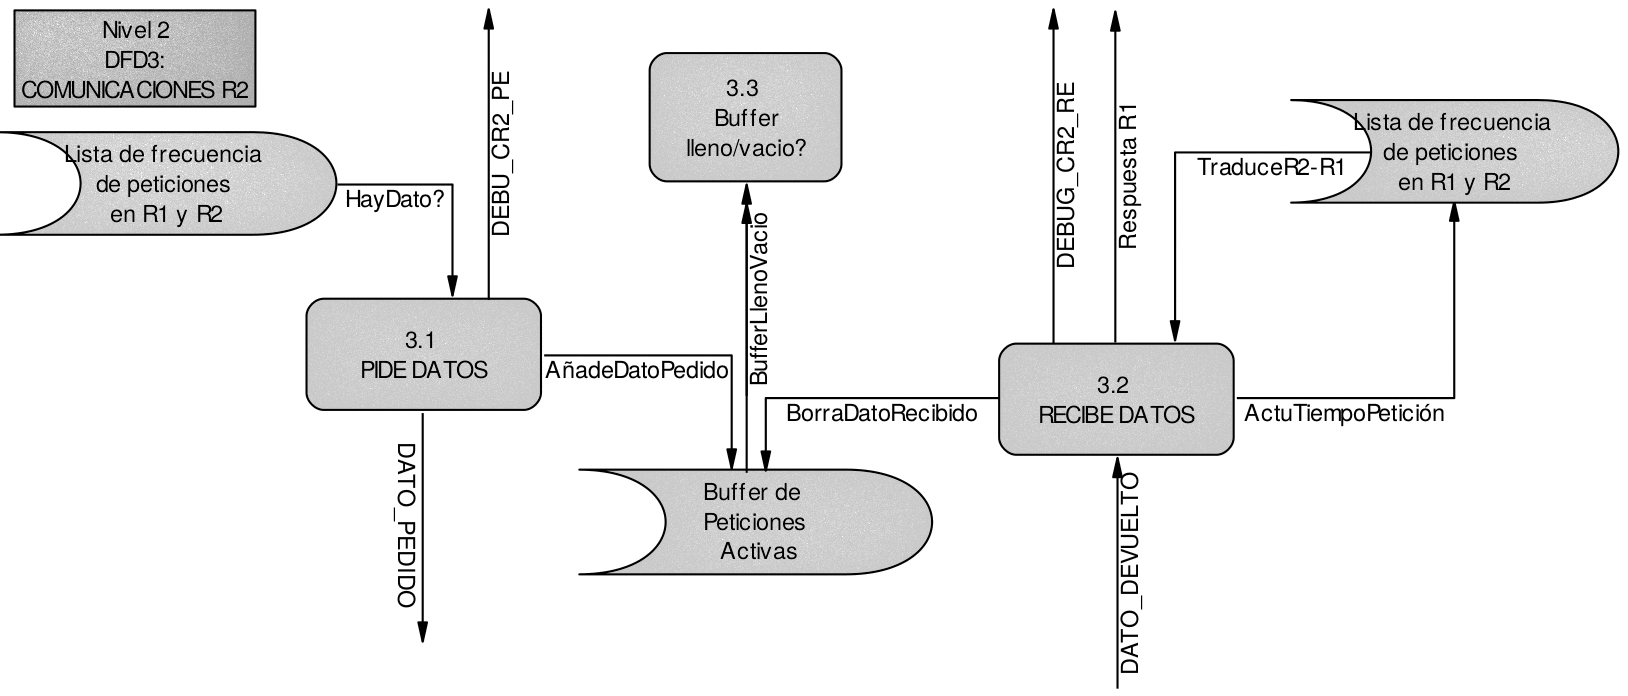
\includegraphics[width=0.7\linewidth]{Resources/Tema5/nivel2_Proceso3_DFD.png}
              \caption{DFD de nivel 2 del proceso $3$ del TDC. Nótese cómo el flujo \textit{DEBUG\_CR2} se vuelve a decomponer incluso más.}
              \label{fig:dfdn2}
          \end{figure}
    \item \textbf{Nivel N}\\
          Contiene los procesos primitivos, que no se pueden descomponer. Para describirlos, deben emplearse técnicas de especificación de procesos.
    \item \textbf{Procesos primitivos}
\end{enumerate}

\textbf{Nota:} \textit{Como se puede observar, un DFD puede dar lugar, como máximo, a tantos DFDs como procesos contenga.}\\

La descomposición de un sistema en diferentes niveles (jerarquía de DFDs) debe respetar la \uline{regla del balanceo}. Sus restricciones pueden separarse en dos partes.\\

En primer lugar, los procesos en el DFD tienen un \textbf{identificador numérico} de modo que:
\begin{itemize}
    \item Nivel 0: Solo contiene un proceso, el \textbf{``0''}
    \item Nivel 1: Se le asigna a cada proceso un número secuencialmente, \textbf{\{1, 2, 3\ldots\}}
    \item Niveles 2...N: La numeración de los procesos en el DFD hijo se deriva del número del DFD padre; \textit{por ejemplo: para el proceso 3, serían 3.1, 3.2\ldots}
\end{itemize}

Por otra parte:

\begin{itemize}
\item El título del DFD hijo debe ser el nombre del proceso que desarrolla.

\item Debe mantenerse la \textbf{consistencia de los flujos de datos entre los DFDs} padre e hijo.
\begin{itemize}
    \item En el diagrama hijo, estos flujos tendrán un extremo libre, puesto que conectaban el proceso padre con algún elemento que ya no va a estar representado. De todos modos, esto no sucede con los flujos que conectan los procesos con los almacenes de datos, en dónde estos últimos sí son representados.
    \item Además, esta regla del balanceo contempla otras excepciones. Un ejemplo de ello lo son los flujos de datos bidireccionales y los compuestos, dado que cada uno de estos deberá descomponerse en algún momento en varios flujos, rompiendo la correspondencia 1 a 1 entre flujos padre e hijo.
\end{itemize}
\end{itemize}

\subsection{Especificaciones de proceso (PSPEC)}

Los DFDs no indican nada acerca de los detalles de cómo se realizan las transformaciones en el sistema. Es aquí en donde entra en juego la \textbf{P}rocess \textbf{Spec}ification, que es un documento que describe textualmente los detalles de un proceso, indicando \textbf{cómo es el procedimiento de transformación de una información de entrada en otra de salida}; dicho de otro modo, debe definir, de forma más o menos formal, cómo se obtienen los flujos de salida a partir de los de entrada más una posible información local.\\

Para generar estos documentos, los procesos de los DFDs de menor nivel (más altos en la jerarquía) se irán describiendo mediante nuevos DFDs, hasta alcanzar un nivel en el que un proceso pueda ser descrito textualmente de forma sencilla y no ambigua; estos procesos suelen llamarse \textbf{procesos primitivos}. De este modo, las PSPEC servirán para complementar los DFDs.\\

Las descripciones de estos procesos deben:

\begin{itemize}
    \item Ser \textbf{breves} (menos de una página).
    \item Incluir \textbf{precondiciones} y \textbf{postcondiciones}.
\end{itemize}

Y, para su elaboración, se utilizan diferentes \uline{técnicas de especificación}:

\begin{enumerate}
    \item Lenguaje natural; \textit{por ejemplo: mediante una definición como ``invertir una matriz''}.
    \item Diagramas de flujo.
    \item Lenguaje estructurado, y diagramas de acción (pseudocódigo, especificar un algoritmo). 
    \item Árboles de decisión.
    \item Tablas de decisión.
\end{enumerate}

\begin{figure}[h!]
    \centering
    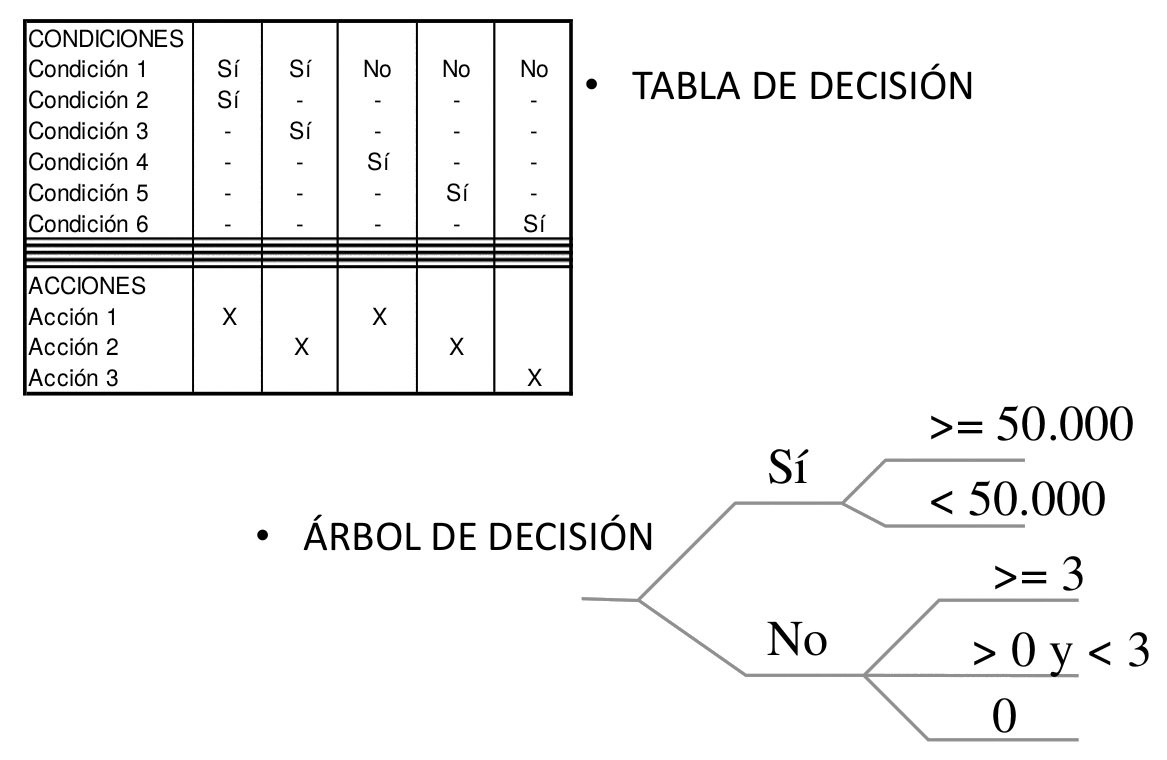
\includegraphics[width=0.6\linewidth]{Resources/Tema5/ejemplosPSPEC.png}
    \caption{Ejemplos de dos PSPEC mediante (1) una tabla de decisión y (2) un árbol de decisión.}
    \label{fig:ejemplosPSPEC}
\end{figure}

\subsection{Estrategia de creación de DFDs y PSPECs}

\begin{enumerate}
    \item \textbf{Diagrama de contexto}:
    \begin{enumerate}
        \item Localizar todas las entidades.
        \item Definir sus flujos con precisión (interfaces).
    \end{enumerate}
    \item \textbf{Diagrama de sistema}:
    \begin{enumerate}
        \item Seleccionar las funciones principales.
        \item Definir los flujos entre dichas funciones; normalmente, a través de almacenes.
        \item Recoger los flujos del diagrama de contexto; normalmente, cada uno entrará en un proceso distinto, y no conviene dividirlos aunque sean flujos múltiples.
    \end{enumerate}
    \item \textbf{Resto de diagramas}:
    \begin{enumerate}
        \item No descomponer al máximo.
        \item Subfunciones principales de cada proceso, e interfaces entre sus procesos resultantes.
        \item Se recogen los interfaces (flujos) de nivel superior y se asignan a alguno de los procesos.
        \item Se pueden desglosar flujos múltiples.
    \end{enumerate}
    \item \textbf{Procesos primitivos}:
    Detenerse cuando:
    \begin{enumerate}
        \item La función puede expresarse en una página.
        \item Los procesos tienen pocos flujos de E/S.
        \item Descomponer implica perder el significado de la función; es decir, se obtienen diagramas demasiado sencillos que complican la compresión global o, dicho de otro modo, que dificultan entender para qué va a servir la función.
    \end{enumerate}
\end{enumerate}


\subsection{Diagramas de flujo de control (DFC, Tiempo--Tiempo)}

Dado que en los DFDs no se representa explícitamente el control o flujo de sucesos del sistema (\uline{cuándo se realizan los procesos o en qué orden}), hay determinados sistemas de software en donde se podrá intuir, pero habrá otros en que \uline{no será posible}. A la hora de \textbf{interpretar el comportamiento de un sistema}, se pueden encontrar \textbf{tres situaciones posibles}:

\begin{itemize}
    \item \textbf{Los procesos que figuran en el DFD están activos siempre}. Por ende, no es necesario especificar el control del sistema.
    \item \textbf{Los procesos se activan cuando llegan datos a través de los flujos de entrada}, los transforman y emiten los resultados a través de los flujos de salida, y \textbf{permanecen inactivos hasta la llegada de nuevos datos}. Este comportamiento está implícito en la notación usada.
    \item \textbf{Cada proceso pasa por períodos de actividad e inactividad}, gobernados por \uline{mecanismos más complejos}. Este tipo de situaciones no pueden representarse debidamente en un DFD, por lo que debe crearse un modelo adicional en donde se representen las \uline{señales de control no implícitas en el DFD}.
\end{itemize}

\textbf{Nota:} \textit{El modelo de control del sistema establece el comportamiento de éste a alto nivel, indicando \uline{qué procesos están activos en cada momento o en qué secuencia se realiza la transformación de los datos}. Existe un control de bajo nivel referido a los saltos condicionales y a los bucles, que estaría reflejado en las PSPECs de los procesos.}\\

Para modelar el control del sistema, se emplearán los \textbf{D}iagramas de \textbf{F}lujo de \textbf{C}ontrol (\textbf{DFC}), los cuales consisten en eliminar de los DFDs todo lo relativo a la información de control, y construir una jerarquía de DFCs paralela a la de DFDs. Según esto, se comenzará por el diagrama de contexto, representando en cada par DFD/DFC los mismos procesos y entidades externas, puesto que \uline{representan modelos de la misma parte del sistema con el mismo nivel de detalle, aunque con puntos de vista distintos}.\\

\subsubsection{Elementos}

Las reglas sobre denominación de numeración, relaciones padre--hijo, y balanceo que se aplican a los DFCs \uline{son las mismas} que se establecen para los DFDs.\\

Por otra parte, los elementos que aparecen en un DFC son prácticamente los mismos:

\begin{itemize}
    \item \textbf{Procesos, entidades externas, y almacenes de datos}: Serán los mismos y \uline{tendrán el mismo significado} que en el DFD.
    \item \textbf{Flujos de control}: Se representan mediante trazos discontinuos y modelan el \uline{flujo de información de control en el sistema}. Habrá procesos o entidades externas que generen información de control, y otras que la consuman. Aparte de emplear los flujos entrantes para la activación/desactivación de procesos, un proceso también puede utilizarlos para transformarlos en flujos de salida según la PSPEC correspondiente.
    \item \textbf{Condiciones de datos}: \uline{Flujos de control generados por un proceso del sistema}. Figuran en el DFC y no en el DFD, pero es la PSPEC la que define cómo se calcula su valor a partir de los flujos de entrada del proceso.
    \item \textbf{Almacenes de control}: Se representan igual que los almacenes de datos, pero con trazos discontinuos. Permiten almacenar información de control para ser utilizada posteriormente.
    \item \textbf{Ventanas de especificaciones de control}: Se representan mediante barras, y reciben flujos de control (condiciones de datos junto con flujos de control del exterior), así como los emiten, actuando de este modo como las \uline{transformaciones de flujos de control en el sistema}; dicho de otro modo, dedicen el comportamiento del sistema. Su comportamiento se define en las especificaciones de control (CSPEC). No están etiquetadas, puesto que \uline{todas las ventanas que aparecen en un determinado DFC hace referencia a una única CSPEC} que define cómo se realizan estas transformaciones.
    \item \textbf{Activadores de procesos} Flujos de control especiales que \uline{activan o desactivan procesos} tomando dos posibles valores, \texttt{ON} y \texttt{OFF}. Tienen el mismo nombre que los procesos que controlan, por lo que no suelen representarse en el DFC excepto por fines de claridad. Siguen la jerarquía de los modelos, es decir: un proceso está activo si, y sólo si todos sus antecesores están activos.
\end{itemize}

\begin{figure}[H]
    \centering
    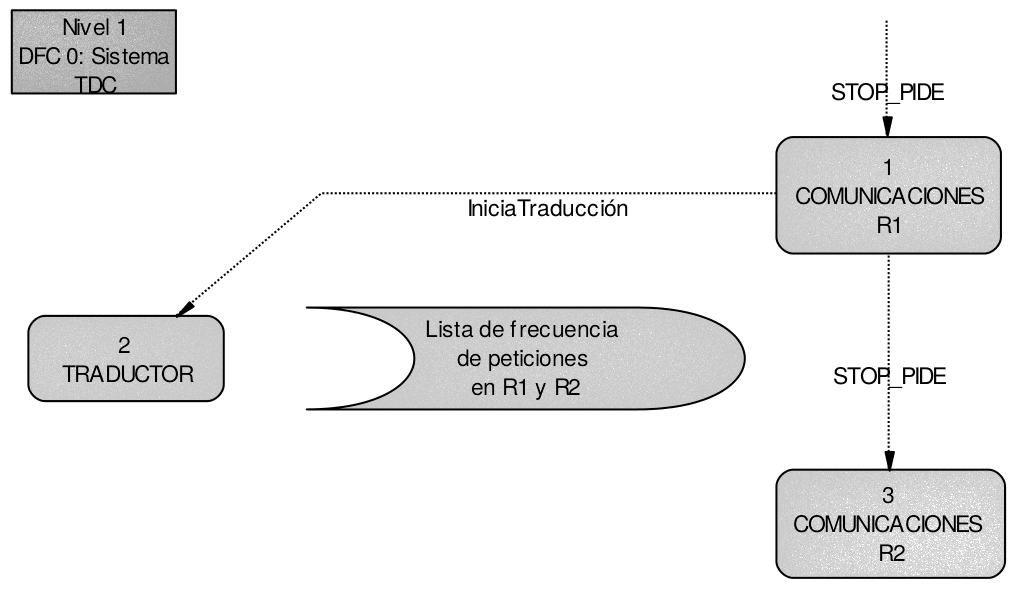
\includegraphics[width=0.8\linewidth]{Resources/Tema5/nivel1_DFC.png}
    \caption{DFC de nivel 1 del TDC.}
\end{figure}

\begin{figure}[H]
    \centering
    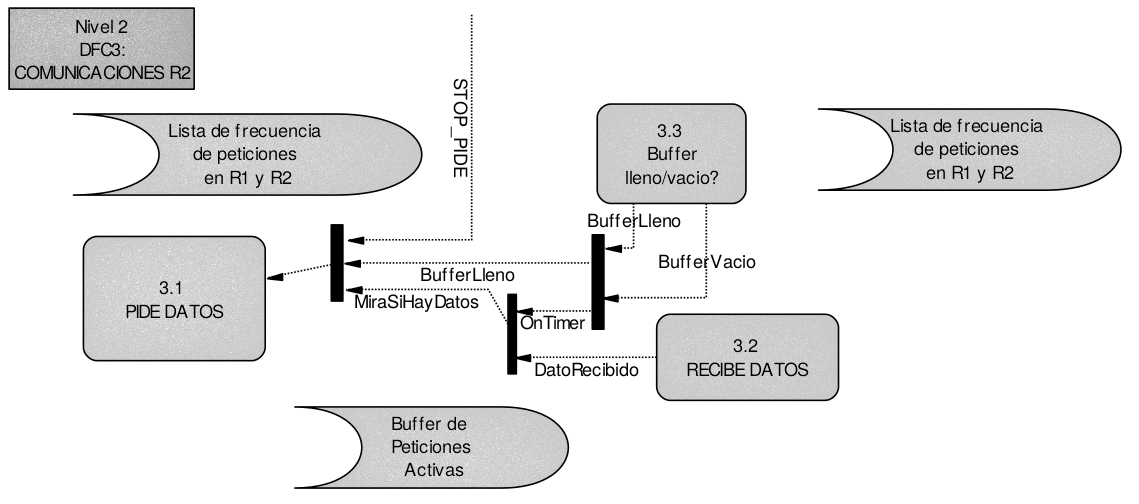
\includegraphics[width=0.9\linewidth]{Resources/Tema5/nivel2_Proceso3_DFC.png}
    \caption{DFC de nivel 2 correspondiente al proceso $3$ del TDC. Nótese la existencia de las condiciones de dato \textit{buffer lleno/buffer vacío}, y del activador entrante en el proceso \textit{3.1 PIDE DATOS}.}
\end{figure}

\textbf{Nota:} \textit{Conviene recordar que, mediante los flujos de control, se define cómo se activan o desactivan los procesos.}\\

\textbf{Nota:} \textit{Dado que los modelos del sistema tienen estructura jerárquica, se considera que un proceso está activo \textbf{solo si todos sus antecesores están activos}. Un proceso que no tiene activador se considera, por lo tanto, activo siempre que sus antecesores lo estén; en caso de tener activador, éste debe tenerse también en cuenta.}\\

\textbf{Nota:} \textit{Los procesos en un DFC indican cómo fluyen los flujos de control a través de ellos. \uline{No representan los estados del sistema} (se encargan los DEs), y \uline{tampoco representan procesamiento ni transformación de los flujos de control} (se encargan las CSPECs).}\\

\textbf{Nota:} \textit{Los DFCs reflejan la información de control que existe en el sistema, y qué procesos y entidades las producen y consumen. Deben ser \uline{combinados} con las CSPECs para reflejar el comportamiento del sistema.}\\

Otro detalle importante es que un flujo de control que entra en un proceso no indica necesariamente que ese proceso se active; la \uline{activación y desactivación de procesos se indica en las CSPECs}. Por lo tanto, un flujo de control entrante puede indicar que:

\begin{itemize}
    \item O bien va a ser utilizado como un dato más para que el proceso lleve a cabo su transformación.
    \item O bien va a ser utilizado para controlar alguno de los procesos en los que se descompone el proceso.
\end{itemize}

\subsubsection{Cómo separar datos y control}

No existen unas normas estrictas para separar, de entre todos los flujos de información, los datos del control. Por norma general, \textbf{se modelarán como señales de control únicamente aquellas que intervengan en la activación y desactivación de algunos de los procesos del sistema de forma no trivial}, mientras que el resto de la información se modelará como datos.\\

En determinadas situaciones, \uline{es posible que un elemento de información determinado se emplee como dato en un proceso y como control en otro}. Para ello, se modelará como dato (trazo continuo) en el DFD, y como control (trazo discontinuo) en el DFC, pero se asignará el mismo nombre a ambos flujos para mostrar que son el mismo.

\subsubsection{Cuándo usar especificaciones de control}

Lo ideal es utilizar DFDs siempre que sea posible, puesto que son más sencillos de realizar y de entender; por ejemplo, el uso de DFCs obligará a mirar en paralelo a los DFDs.\\

En todo caso, debe recordarse siempre que es necesario centrarse en el \textbf{modelo abstracto o lógico} del sistema, mientras que las especificaciones ya tratarán los aspectos de más bajo nivel.

\subsection{Especificaciones de control (CSPEC)}

Son similares a las PSPECs, ya que en ambos casos se definen los detalles procedimentales de cómo se realiza el procesamiento de los flujos de entrada y salida. Sin embargo, hay una diferencia importante entre PSPECs y CSPECs:

\begin{itemize}
    \item Las PSPECs se utilizan para describir las primitivas de proceso.
    \item Las CSPECs sirven para modelar el comportamiento de un DFC, describiendo cómo se procesan los flujos de control. Por lo tanto, habrá, como máximo, una CSPEC por cada DFC de la jerarquía, ya que el primero determina la activación del segundo, utilizando las \textbf{ventanas de control del DFC como interfaces}.
\end{itemize}

Así, se puede concretar que una \textbf{C}ontrol \textbf{SPEC}ification es un documento que \textbf{especifica el comportamiento un DFC} (y, por lo tanto, del sistema). Concretamente, se indica cómo, a partir de las señales de control que entran en una ventana, se determina la activación o desactivación de los procesos comprometidos.\\

Estas CSPECs pueden caracterizarse mediante:

\begin{itemize}
    \item \textbf{Lenguaje estructurado} (pseudocódigo).
    \item \textbf{Sistemas combinacionales} (el valor de salida se determina exclusivamente a partir de los valores de entrada):
    \begin{itemize}
        \item Tablas de decisión: Indican cómo calcular las señales de salida en función de las de entrada.
        \begin{table}[h!]
            \centering
            \resizebox{0.4\textwidth}{!}{%
                \begin{tabular}{|l|c|c|c|c|c|}
                    \hline
                    \multicolumn{6}{|c|}{\textbf{CONDICIONES}} \\ \hline
                    Condición 1 & Sí & Sí & No & No & No       \\
                    Condición 2 & Sí & -  & -  & -  & -        \\
                    Condición 3 & -  & Sí & -  & -  & -        \\
                    Condición 4 & -  & -  & Sí & -  & -        \\
                                &    &    &    &    &          \\ \hline
                    \multicolumn{6}{|c|}{\textbf{ACCIONES}}    \\ \hline
                    Acción 1    & X  &    & X  &    &          \\
                    Acción 2    &    & X  &    & X  & X        \\\hline
                \end{tabular}
            }
            \caption{Ejemplo de tabla de decisiones de un proceso.}
        \end{table}
        \item Tablas de activación de procesos: Similares a las anteriores, pero indicando para cada proceso del DFC si está activo o no ante cada combinación.
    \end{itemize}
    \item \textbf{Sistemas secuenciales}:
    \begin{itemize}
        \item Diagramas de Estados: Autómatas finitos.
        \begin{figure}[h!]
            \centering
            \includegraphics[width=0.9\linewidth]{Resources/estados}
            \caption{Ejemplo de un diagrama de estados.}
        \end{figure}
        \item Redes de Petri: Técnica muy apropiada en el caso de tratar con sistemas de comportamiento asíncrono concurrente.
        \begin{figure}[H]
            \centering
            \includegraphics[width=0.75\linewidth]{Resources/redPetri}
            \caption{Proceso de generación de una reclamación modelado en redes de Petri.}
        \end{figure}
    \end{itemize}
\end{itemize}

\subsection{Estrategia de creación de DFCs y CSPECs}

\begin{enumerate}
    \item Construir una jerarquía de DFCs paralela a la de DFDs.
    \item Cada par DFC/DFD representa los mismos procesos y las mismas entidades externas.
    \item Solo se introducen las señales de control que no estén implícitas en el DFD.
    \item Cada DFC se desarrolla en un CSPEC, siempre y cuando se considere necesario.
\end{enumerate}

\begin{figure}[H]
    \centering
    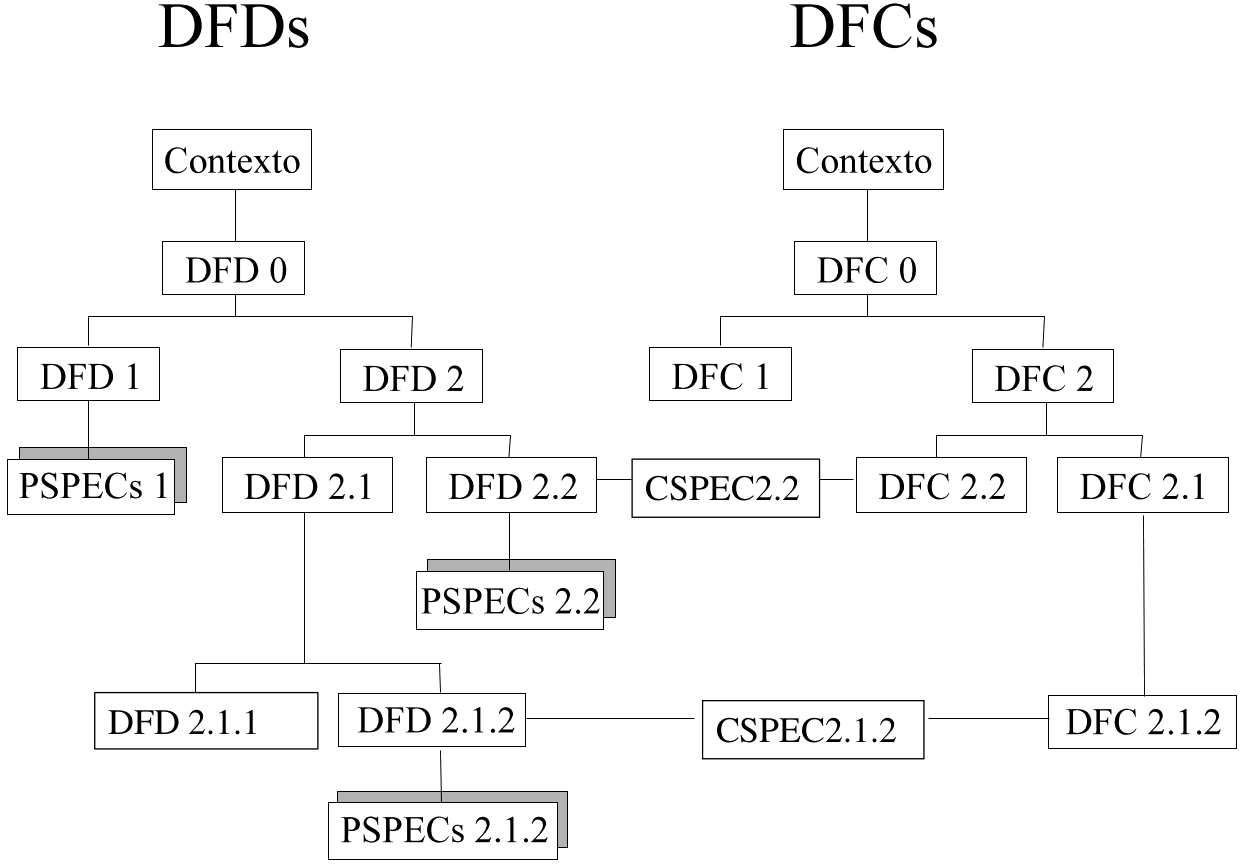
\includegraphics[width=0.8\linewidth]{Resources/Tema5/jerarquiaDFCs.png}
    \caption{Ejemplificación de la jerarquía de DFCs paralela a la de DFDs.}
\end{figure}

En resumen, por cada DFD se crea un DFC gemelo si alguno de los procesos del DFD genera o consume información de control. Además, si alguno de los procesos del DFD es activado o desactivado de forma no implícita, éste DFC llevará una ventana de control y se hará una CSPEC para indicar cuándo se realiza la activación y desactivación.

\subsection{Diagramas Entidad--Relación (DER)}

Los \textbf{D}iagramas \textbf{E}ntidad--\textbf{R}elación resuelven las insuficiencias que se pueden producir en la representación de datos complejos mediante los almacenes en los diagramas de flujo de datos (DFD). Para ello, no solo se muestra la información contenida, sino también las relaciones que existen entre los propios datos.

\begin{figure}[H]
    \centering
    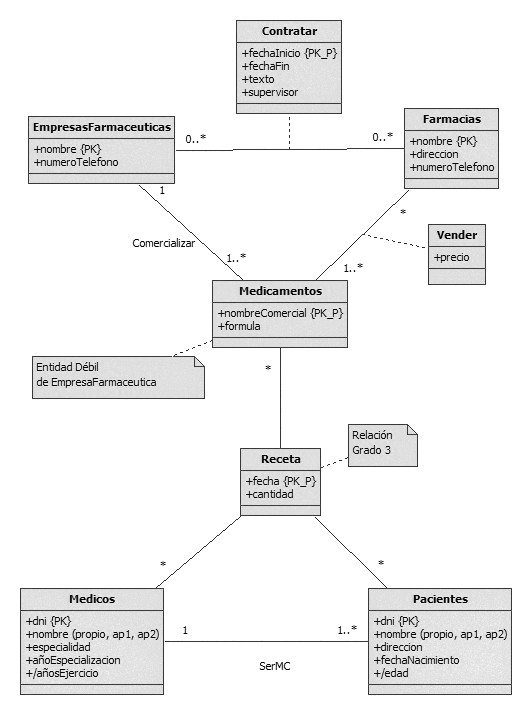
\includegraphics[width=0.6\linewidth]{Resources/Tema5/Caso12_RecetasRayosX_MER.jpg}
    \caption{Ejemplificación de un Diagrama Entidad--Relación.}
\end{figure}

\subsection{Comprobaciones}

Una vez esté realizada la especificación estructurada, debe comprobarse si cumple las siguientes propiedades:

\begin{enumerate}
    \item \textbf{Compleción}: Los modelos son completos.
    \item \textbf{Integridad}: No existen contradicciones ni incoherencias entre los modelos.
    \item \textbf{Exactitud}: Los modelos cumplen los requisitos del usuario.
    \item \textbf{Calidad}: Presencia de estilo, legibilidad y facilidad de mantenimiento.
\end{enumerate}

\textbf{Nota:} \textit{Es recomendable realizar las comprobaciones elaborando una checklist en la que se comprueben, con profundidad, aspectos sobre todas estas propiedades.}

\subsection{Consistencia entre modelos}

El conjunto de modelos tiene como misión dar una visión global del sistema, desde diversos puntos de vista; por lo tanto, representan siempre el mismo sistema, así que deben ser consistentes.\\

Las técnicas matriciales se utilizan \textbf{principalmente para ayudar a verificar la consistencia entre los componentes de distintos modelos} de un sistema, ya sean centrados en la dimensión de las funciones, en la de la información, o en la temporal.

\begin{enumerate}
    \item \textbf{Matriz Entidad/Función}: Visualiza las relaciones existentes entre las funciones que lleva a cabo un sistema y la información necesaria para soportarlas.\\
    
    Los elementos de las filas son entidades o relaciones presentes en el DER, mientras que los de las columnas pueden ser funciones de alto nivel representadas en un DFD.\\

    En cada celda se incluyen las \textbf{acciones} que puede realizar la función (\textbf{I}nsertar, \textbf{L}eer, \textbf{M}odificar y \textbf{B}orrar).

    \begin{table}[h!]
        \centering
        \begin{tabular}{cl|c|c|c|} \cline{3-5}
                                                                                                    &                                   & \multicolumn{3}{c|}{\textbf{Funciones}}                              \\ \cline{3-5}
                                                                                                    &                                   & Gestionar Presupuesto                   & Gestionar Cliente & \ldots \\ \cline{2-5}
            \parbox[t]{2mm}{\multirow{3}{*}{\rotatebox[origin=c]{90}{{\small \textbf{Entidades}}}}} & \multicolumn{1}{|c|}{Cliente}     & L                                       & I, M, B           &        \\ \cline{2-5}
                                                                                                    & \multicolumn{1}{|c|}{Presupuesto} & I, M, B                                 &                   &        \\ \cline{2-5}
                                                                                                    & \multicolumn{1}{|c|}{\ldots}      &                                         &                   &        \\ \cline{2-5}
        \end{tabular}
        \caption{Ejemplo de Matriz Entidad/Función.}
        \label{tab:matrizEF}
    \end{table}

    \item \textbf{Matriz Entidad/Entidad}: Muestra las relaciones habituales del DER, indicando en cada celda la relación entre las entidades implicadas. Es de utilidad, sobre todo, cuando se presenta un número alto de entidades.
          
          \begin{table}[h!]
              \centering
              \begin{tabular}{cl|c|c|c|} \cline{3-5}
                                                                                                          &                                   & \multicolumn{3}{c|}{\textbf{Entidades}}                        \\ \cline{3-5}
                                                                                                          &                                   & Cliente                                 & Presupuesto & \ldots \\ \cline{2-5}
                  \parbox[t]{2mm}{\multirow{3}{*}{\rotatebox[origin=c]{90}{{\small \textbf{Entidades}}}}} & \multicolumn{1}{|c|}{Cliente}     &                                         & Tiene       &        \\ \cline{2-5}
                                                                                                          & \multicolumn{1}{|c|}{Presupuesto} &                                         &             &        \\ \cline{2-5}
                                                                                                          & \multicolumn{1}{|c|}{\ldots}      &                                         &             &        \\ \cline{2-5}
              \end{tabular}
              \caption{Ejemplo de Matriz Entidad/Entidad.}
              \label{tab:matrizEE}
          \end{table}

          %mecago en dios tanto royo para definir señales de control y ahora usa eventos....
    \item \textbf{Matriz Evento/Entidad} (evento $\equiv$ señal de control): Muestra las acciones que provocan los eventos sobre las entidades (datos almacenados): (\textbf{I}nsertar, \textbf{L}eer, \textbf{M}odificar y \textbf{B}orrar).

        \begin{table}[h!]
              \centering
              \begin{tabular}{cl|c|c|c|} \cline{3-5}
                                                                                                        &                                             & \multicolumn{3}{c|}{\textbf{Entidades}}                        \\ \cline{3-5}
                                                                                                        &                                             & Cliente                                 & Presupuesto & \ldots \\ \cline{2-5}
                  \parbox[t]{2mm}{\multirow{3}{*}{\rotatebox[origin=c]{90}{{\small \textbf{Eventos}}}}} & \multicolumn{1}{|c|}{Datos del cliente}     & I, M, B                                 &             &        \\ \cline{2-5}
                                                                                                        & \multicolumn{1}{|c|}{Datos del presupuesto} & I                                       & I, M, B     &        \\ \cline{2-5}
                                                                                                        & \multicolumn{1}{|c|}{\ldots}                &                                         &             &        \\ \cline{2-5}
              \end{tabular}
              \caption{Ejemplo de Matriz Evento/Entidad.}
              \label{tab:matrizEvE}
          \end{table}
\end{enumerate}


\section{Metodología del análisis estructurado}

Una vez vistas todas las anteriores notaciones, se detallará ahora cómo coordinarlas durante el trabajo.

\subsection{Fases}

\subsubsection{Creación del modelo de procesos}

El punto de partida será la creación del modelo de procesos del sistema, modelando el ámbito de información y el funcional mediante DFDs y PSPECs.\\

Inicialmente, debe \textbf{revisarse toda la documentación inicial}; es importante pensar antes de ponerse a dibujar diagramas. Por ejemplo, puede realizarse un \textbf{análisis gramatical} de toda esta información, para facilitar la identificación de muchos de los componentes del sistema:

\begin{itemize}
    \item Las \uline{entidades externas} se corresponderían con los \uline{nombres}.
    \item Los \uline{flujos y almacenes de datos} también se corresponderían con los \uline{nombres}.
    \item Los \uline{procesos} se corresponderían con los \uline{verbos}.
\end{itemize}

Además, la especificación (documentación) estudiada también establecerá las relaciones entre dichos nombres y verbos de por sí. A pesar de que lo obtenido hasta el momento no sea completamente correcto, o esté incompleto, sí marca un buen punto de partida.\\

Tras ello, se comienza a realizar el \textbf{DFD de contexto}, y se va refinando en mayores niveles de detalle siguiendo las \textbf{reglas de construcción}. Es importante respetar las reglas de \textbf{acoplamiento mínimo} entre procesos distintos, y de \textbf{máxima cohesión} dentro de un proceso, así como mantener la \textbf{consistencia} entre los diferentes componentes de la jerarquía de DFDs. También debe recordarse el \textbf{evitar detalles de implementación}, así como \textbf{ir incluyendo en el diccionario de datos (DD) los elementos de los DFDs}.\\

El proceso de descomposición finalizará una vez de \textbf{encuentren los procesos primitivos} (procesos sencillos con máxima cohesión $\equiv$ realizan una única función), y que se describirán mediante \textbf{PSPECs}. Estos últimos no contienen definiciones de datos, por lo que no pueden actuar como almacenes de datos, sino emplear tan solo variables locales, aparte de los datos de entrada.

\subsubsection{Creación del modelo de control}

\textbf{No todos los sistemas requieren modelos de control}, al poder estar esta información presente, a veces, de forma implícita en los DFDs. En caso de realizarse, hay que tener \textbf{especial cuidado en no caer en detalles de implementación}.\\

Esta actividad debe comenzar por \textbf{establecer una jerarquía de DFCs simétrica a la de DFDs}, de modo que cada par DFD/DFC contiene los mismos procesos, almacenes de datos, y entidades externas, y hasta en la misma posición, para facilitar la identificación de estos elementos. A continuación, se \textbf{eliminan del DFD todos los flujos que transporten información de control}, y se representarán en los DFCs.\\

A \textbf{cada par DFD/DFC} en donde el DFD es antecesor inmediato de procesos primitivos, \textbf{le podrá corresponder una CSPEC}; esta puede ser combinacional, secuencial o compuesta, y se escogerá siempre el modelo más sencillo posible. Es importante recordar que debe \textbf{mantenerse la consistencia de flujos entre las ventanas de control y las CSPECs}.

\subsubsection{Creación del modelo de datos}

\textbf{Si los datos que maneja el sistema tienen una estructura compleja}, no bastará con definir en el DD el contenido de cada uno. Se desarrollará en su lugar un modelo de datos empleando \textbf{DERs}, donde se muestren las \textbf{relaciones} que existan entre los datos que maneje el sistema.

\subsubsection{Consistencia entre modelos}

Finalmente, una vez realizados los distintos modelos del sistema, deberían llevarse a cabo todas las \textbf{técnicas de consistencia entre modelos} que se consideren necesarias.


\section{Modelos del sistema}

\subsection{El modelo esencial}

El \uline{modelo esencial} del sistema (algunas veces llamado modelo lógico) representa lo que \textbf{el sistema debe hacer para satisfacer los requisitos del usuario}. Es, por lo tanto, un modelo abstracto que supone que disponemos de una \uline{tecnología perfecta} sin coste alguno.\\

Este modelo es el \textbf{resultado de la fase de análisis de requisitos del sistema}, por lo que debe estar completamente libre de detalles de implementación. Algunos errores típicos al realizarlo son:

\begin{itemize}
    \item \textbf{Secuenciar los procesos del DFD}: Deben ser lo más concurrentes posibles, en lugar de pensar que el sistema realiza las tareas una detrás de otra. El único secuenciamiento que debe aparecer en los DFDs es por la dependencia de datos; cualquier otra secuencia es puramente arbitraria, y dependerá fundamentalmente de necesidades de implementación.
    \item \textbf{Utilizar ficheros temporales o de backup}: Estos se usan para conectar procesos que no pueden ejecutarse simultáneamente por limitaciones de la capacidad del hardware, y no porque deban ejecutarse de forma secuencial. Pero, en este modelo esencial, estamos suponiendo que contamos con una tecnología perfecta con la que evitar este tipo de limitaciones, por lo que no se requiere esta clase de ficheros.
    \item \textbf{Utilizar información redundante o que puede ser derivada}: En el modelo esencial no se usará nunca este tipo de información, ya que tiene más que ver con la eficiencia de implementación que con los requisitos del modelo. \textit{Por ejemplo: un error sería almacenar en una base de datos un dato que podría declararse como derivado, solo por evitar calcularlo cada vez que se requiera}.
\end{itemize}

A partir del modelo esencial, los diseñadores podrán decidir cómo implementar el sistema, usando la \uline{tecnología disponible}.

\subsection{Modelo de implementación}

Sin embargo, lo normal es que el cliente proporcione más información que los requisitos del sistema, y que decida también sobre detalles de implementación: qué funciones serán manuales y cuáles automáticas, el formato de los datos de salida, etc. Toda esta información no se refiere a los requisitos esenciales del sistema, sino a los \uline{requisitos de implementación}, que formarán parte del \uline{modelo de implementación} del sistema.\\

El desarrollo de este modelo es una tarea que está a \textbf{medio camino entre el análisis y el diseño}. No puede ser desarrollado solo por el analista y el cliente, dado que se necesita el consejo de diseñadores e implementadores, ya que conocen la tecnología disponible. Por otra parte, no puede ser realizado únicamente por diseñadores e implementadores, porque el usuario debe definir una gran cantidad de requisitos de información, y es el analista quien los describe, haciendo de vínculo entre el cliente y el equipo de desarrollo.\\

En definitiva, este modelo será una \textbf{versión revisada y anotada del modelo esencial, especificando todos esos detalles adicionales}. Sobre ellos, se puede destacar:

\begin{itemize}
    \item La elección de dispositivos de entrada y salida.
    \item La elección de los dispositivos de almacenamiento.
    \item El formato de las entradas y las salidas.
    \item La secuencia de operaciones de entrada y salida, incluyendo la definición de cómo será el diálogo con el usuario.
    \item El volumen de datos esperado.
    \item El tiempo de respuesta requerido.
    \item La realización de copias de seguridad, y las posibilidades de exportar bajo demanda datos contenidos en el sistema.
    \item La seguridad.
\end{itemize}
